
\chapter{Literature study}
\label{chapter:title}

\section{Question 1}

\section{Question 2}
To adjust our design to the given requirements, there has to be an understanding of the variable of natural frequency. The natural frequency itself is defined by many variables related to both the geometry and the material of a structure. The equation for the determination of the magnitude of the natural frequency is given by;
\begin{equation} \label{natural frequency, q2}
    f_n = \frac{1}{2\pi} \cdot \sqrt{\frac{k}{m}}
\end{equation}
Equation \eqref{natural frequency, q2} consists of the variables m (mass) and k. Here k is the 'stiffness' of the structure. The magnitude of this variable can be approached by dividing the force ($F$) by the accompanying deflection ($\delta$). Hence,
\begin{equation}
    k = \frac{F}{\delta}
\end{equation}
Also, $\delta$ can be defined by the following equation.
\begin{equation}
    \delta = \frac{F \cdot L^3}{48 \cdot E \cdot I}
\end{equation}
With F the force applied, L the length of the structure, E the Young's modulus and I the moment of inertia.
So concluding which variables/parameters govern the natural frequency of a structure, we see that there are two main pillars to which they do contribute. \\
\textbf{Geometry}
\begin{itemize}
    \item Lenght ($L$). This is obviously related to the geometry. \textit{The larger L, the smaller the natural frequency.}
    \item Moment of Inertia ($I$). This has to do with the geometry of the structure. Indirectly, the center of gravity (c.g.) depends the magnitude of I. In general, \textit{the farther away the c.g. is from the rotating axis, the larger the moment of inertia.} This is true when the considered structure is made of one single material.
\end{itemize}
\textbf{Material}
\begin{itemize}
    \item Mass ($m$). The magnitude depends on the density of the material and thus the mass is a mainly a material property.
    Of course, the mass could also be categorised in the geometry part (the volume used). \textit{The larger the mass, the smaller the natural frequency.}
    \item Young's modulus ($E$). Every type of material has a different Young's modulus. These typically range from $10^-4$ up to $10^3$ GPa. \textit{The larger the Young's modulus, the smaller the natural frequency.}
\end{itemize}
So concluding, the natural frequency of a structure depends on several (in)dependent properties which are either related to the choice of geometry or the choice of material.

\section{Question 3}
When the temperature of the atmosphere of the different planets increases, the stiffness of the material will decrease. This way, for planets with high temperatures we need materials with a high yield stress. Equally, when the temperature is really low, the material has a high change of cracking so we need a high fracture toughness.

When a planet has a high gravity constant, the gravity force of the rover will increase. By the formula 
\begin{equation} \sigma = \frac{F}{A}
\end{equation}
We can conclude that we need a higher stiffness for a bigger force, so we need a material with a high yield strength.
The change in design parameters also depends on the surface of the planet. When the surface has, for instance, a though surface with lots of rocks and dust, we need wheels with a lot of grip and high fracture toughness, so the wheels won't crack. 

When a planet has a lot of ultraviolet light from for example the sun or an other nearby star, there will occur UV degradation on the material. The absorbed energy can excite photons in plastic and these can create free radicals. In the presence of radical receptors on the planet, the material can crack. On planets with a lot of UV light, it is therefore best to not use plastic. Also high energy waves(radiation) can effect the materials and even the instruments of the rover, however this will only be a problem it there is a lack of atmosphere. This is a significant problem in environments like the Moon and Mars


-Atmospheric composition
Other planets bring different atmospheres, a consequence of a different atmosphere is that it can be a very hostile environment for the rover. As a result the composition of the atmosphere has to be accounted for. A atmosphere can contain different gasses that all have different effects on the materials of the rover. 
One form of corrosion is caused by oxygen that is dissolved in water, so if the atmosphere is very dry this will not be a problem but when the atmosphere is humid this could seriously affect the material by corrosion. 
Another form of corrosion is metal dusting. This occurs when there is a presence of carbon mono-oxide, however at temperatures below 300 degrees this is very insignificant only at very high temperatures above 300 degrees this rusting has to be taken in to account.
Some  metals such as stainless steel and aluminium alloys also rust in the presence of chloride but also in this case there has to be a presence of water. 
Corrosion rates are also very much influenced by conditions as humidity, temperatures and the presence of contaminants such as Chlorides. So when going on a mission to another planet this all has to be looked in to. Corrosion can be prevented by treating the metal or choosing a metal that won't easily corrode.



\section{Questions 4,5}

Nowadays, many governments and companies produce rockets so there is a wide variety of data that all these rockets have. In order to calculate the expected launch loads on the Rocker Bogie a selection of 4 commonly-used rockets is made: Soyuz (Russia), Falcon 9 (SpaceX, USA), Ariane 5 (Europe) and Atlas 5 (USA).

\begin{figure}[h!]
\centering
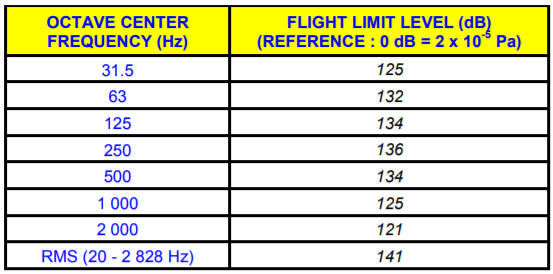
\includegraphics[width=8cm]{figures/Soyux_vibra.png}
\caption{Soyuz vibrations}
\label{Soyuz vibrations}
\end{figure}

\begin{figure}[h!]
\centering
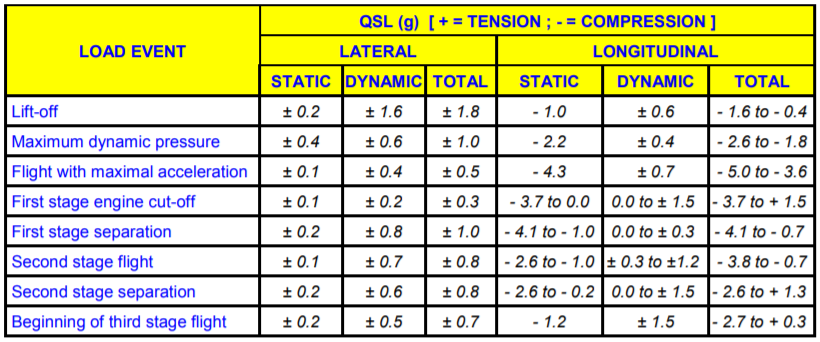
\includegraphics[width=8cm]{figures/Soyuz_acce.png}
\caption{Soyuz acceleration}
\label{Soyuz acceleration}
\end{figure}


\begin{figure}[h!]
\centering
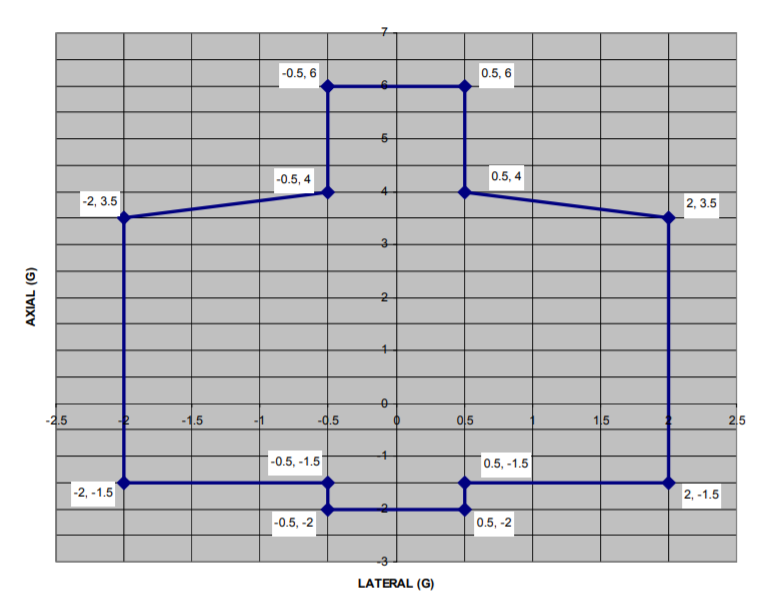
\includegraphics[width=8cm]{figures/Falcon9_acc.png}
\caption{Falcon 9 acceleration}
\label{Falcon 9 acceleration}
\end{figure}

\begin{figure}[h!]
\centering
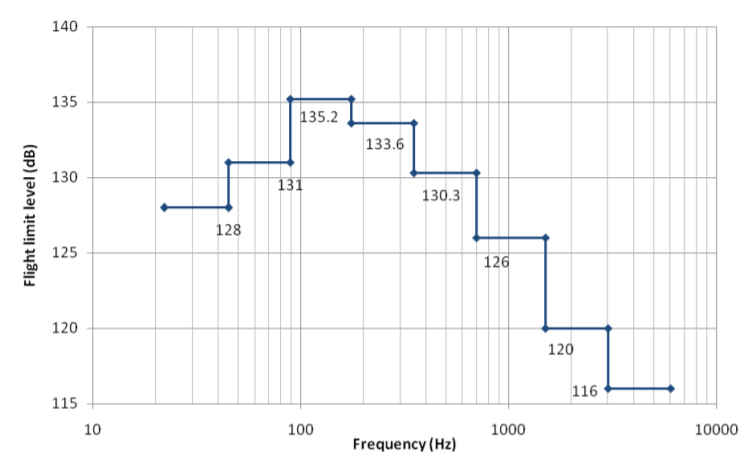
\includegraphics[width=8cm]{figures/Falcon9_vibr.png}
\caption{Falcon 9 vibrations}
\label{Falcon 9 vibrations}
\end{figure}

\clearpage

\begin{figure}[h!]
\centering
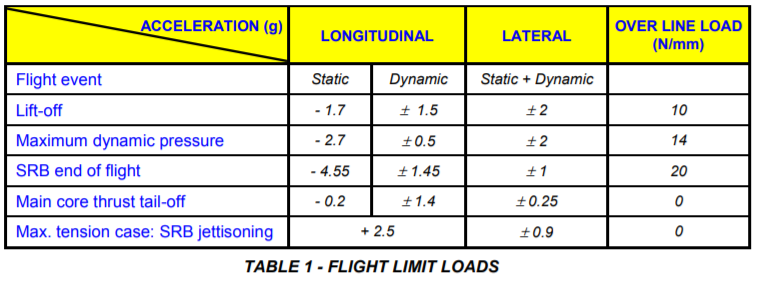
\includegraphics[width=8cm]{figures/Ariane5_acc.PNG}
\caption{Ariane 5 acceleration}
\label{Ariane 5 acceleration}
\end{figure}

\begin{figure}[h!]
\centering
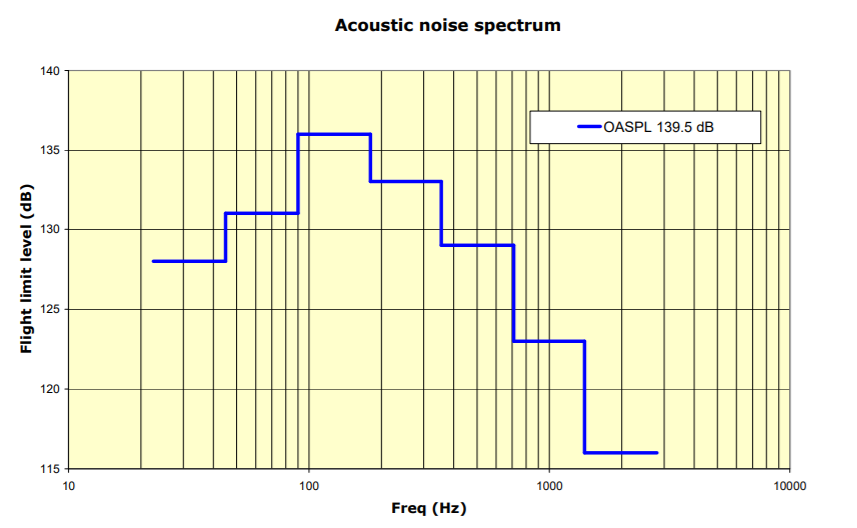
\includegraphics[width=8cm]{figures/Ariane5_Vibr.png}
\caption{Ariane 5 vibrations}
\label{Ariane 5 virbrations}
\end{figure}

\begin{figure}[h!]
\centering
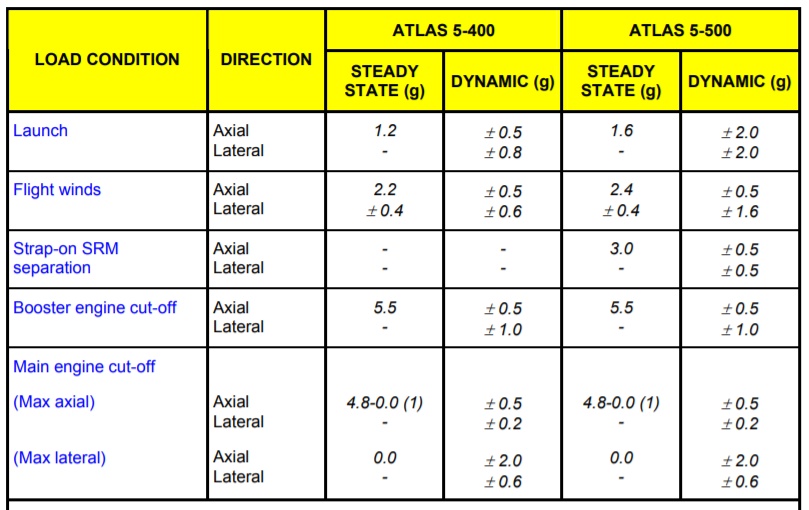
\includegraphics[width=8cm]{figures/Atlas5_acc.PNG}
\caption{Atlas 5 acceleration}
\label{Atlas 5 acceleration}
\end{figure}

\begin{figure}[h!]
\centering
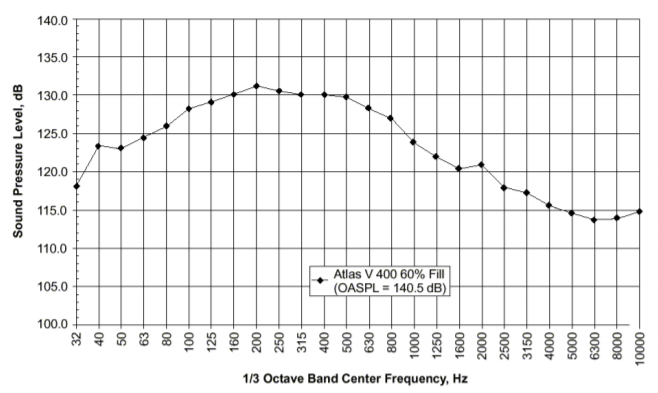
\includegraphics[width=8cm]{figures/Atlas5_vibr.PNG}
\caption{Atlas 5 vibrations}
\label{Atlas 5 virbrations}
\end{figure}

Considering all this data an assumption can be made about what launch loads the Rocker Bogie should withstand. By examining these examples we can conclude that generally the static loads are between 4-6g at peak loading which is at booster engine cut-off. At this peak loading the Rocker Bogie should be able to withstand a load 4 to 6 times its own weight relative to that on Earth.
\\

At the same time the Rocker Bogie should also coop with the frequencies released during flight. The spectrum of frequencies are shown in figures 2.1, 2.4, 2.6 and 2.8. Frequencies like these create stresses in the materials which can over time create fatigue loading.



\section{Question 6}

\section{Question 7}

The bending stiffness of a beam (EI), can be derived from the formula of the spring constant in lateral direction.
\begin{equation}
    k_y= \frac{3EI}{L^3}
\end{equation}
This formula can be rewritten in the form:
\begin{equation}
    EI=\frac{L^3 \cdot k_y}{3}
\end{equation}
Where L is the length of the beam and $k_y$ is the spring constant. With this formula you can caluculate the bending stiffness of a aluminium beam. For a fully composite beam we need 
\section{Question 8}

The structure of the rocker bogie has to withstand dynamic loads, such as heavy vibrations, during launch. After landing the vertical beams in the structure as seen in [reference to sketch from project manual]are loaded in compression and the horizontal ones in bending as it supports the weight of rest of the vehicle. Whilst withstanding the different load cases, EDD*E, the universal planet reconnaissance vehicle which the rocker bogie structure supports, must properly function during operation on different planetary surfaces with different environmental conditions.
\\
\\
(properly referenced sketch from project manual)     !!!!
\\
\\
When analysing the primary loads during launch, most will largely be of influence on the launch [maybe reference these pages in the m&s reader] vehicle, not the payload. ]The payload, in this case EDD*E, will however be subject to quite severe vibrations. Cyclic loading such as this can result in failure, usually in the form of fatigue damage. Metals such as aluminium initially respond to vibrations by strain hardening, increasing the strength of the material. It takes long for cracks to propagate and reach a critical crack length (maybe reference to these pages in the materials book)      !!!!     . Strain hardening in composites is negligible making the phase in which the crack propagates much shorter than for aluminium. Once sufficient damage is available in the material, it progresses to failure fairly quickly. On the other hand, composites do offer certain vibration damping properties which, in one way, can be achieved by the addition of vibration damping material. Even though it solves the vibration problem, these processes do add weight to the final structure and are expansive to manufacture. 
\\
\\
Another danger of the vibrations during launch is if the rocker bogie structure were to approach its natural frequency. Oscillations increase drastically if that were to happen. To ensure the safety of the rocker bogie, its natural frequency should be well above the frequency of the vibrations caused by the launch vehicle. As given in (reader structures and materials reference)      !!!!!      the equation for the natural frequency of a mass spring system is the following:
\\
\\
(equation natural frequency)     !!!!!
\\
\\
It shows that the natural frequencies can be increased by decreasing the mass of the structure. Composites generally have lower densities than aluminium alloys as can be seen in (reference to picture bubble chart rho-E materials book)    !!!!!
\\
\\
(properly referenced picture materials book)     !!!!!
\\
\\
Assuming the dimensions of the structure will remain about the same, regardless of which material is used. A structure made out of composites would have a lower mass and thus a higher and safer natural frequency. The structure can however be designed properly so as to stay in a safe range of frequencies even when using the heavier aluminium.
\\
\\
A higher mass decreases the natural frequency. This shows a part of the general main objective in aerospace design of the minimization of weight. A part of weight minimization comes from the objective of cost minimization. A lighter structure of the same material means saving up on material costs, since less is needed to produce the structure. Composites have a very positive stiffness-to-weight ratio, considerably better than aluminium. For the same required stiffness, composite structures are lighter than aluminium, an obvious advantage. Opposite of that composites do have high production costs considering that the production is very complicated and labour-intensive. Aluminium however, has great manufacturability. It’s quite cheap and easy to apply production processes like forming or machining. Even though composites do have adequate workshop properties, they get much harder to cut by machining when the strength of e.g. the fibres increases. To be able to machine composites, the strength is partially sacrificed by using weaker fibres, which is an undesirable result.
\\
\\
On another note; after EDD*E has landed on a planetary surface it is more prominently subjected to different loading cases. The simple design of the rocker bogie structure consists of multiple beams mostly loaded in either compression (The vertical beams) or bending (The horizontal beams). By placing a hinge at both positions A and B (reference to sketch from project manual)      !!!!     , the bending loads in the horizontal beams are partially prevented leaving the most prominent loading case to be the compression in the vertical beams. Composites are anisotropic and even though they’re a great choice for when the main load case is uniaxial tension, they’re not ideal when loaded in compression. Aluminium is isotropic, it can be loaded in any direction and has similar strength in both tension and compression. Therefore compressive loads, as present in part of the rocker bogie structure, can have destructive results when it’s made out of composites whilst it will generally lead to very little to no damage in metals such as aluminium.
\\
\\
For EDD*E to be able to function properly on different planetary surfaces, the conditions in which it has to operate can differ greatly. The structure of the rocker bogie is required to withstand certain loads during operation, specific operating conditions can negatively influence the structures properties, e.g. reducing the strength of the material. 
\\
\\
The possible operating conditions on the different planetary surfaces may include a large range of temperatures in which it must be able to operate. All engineering materials, thus including both composites and aluminium, show some temperature dependent behaviour. An increase in temperature often leads to material properties deteriorating. The range of safe operating temperatures are influenced by many different factors and both aluminium and composites can be modelled towards a positive operating temperature window.
\\
\\
As can be read in (reference to totalmateria article)     !!!!!!      the properties of aluminium don’t change as drastically as some other materials when it undergoes a change in temperature. Aluminium has no ductile-to-brittle transition, therefore it stays tough even at lower temperatures leading up to almost  -200 degrees Celsius (cryogenic). As the temperature increases, aluminium doesn’t intrinsically keep it’s strength, but by using methods such as solid-solution strengthening, second phase hardening and the use of rapid solidification technology, there is the possibility to create aluminium that show promise for operating at temperatures up to 350 degrees Celsius.
\\
\\
Composites, however, show much more drastic changes in their properties as the temperature is either increased or decreased as is described in [reference to Cambridge document]. Considering that composites are made of multiple different materials, these all show a different reaction to the temperature change. The materials will either contract or expand which results in internal stresses and even a separation of the reinforcement and matrix e.g. delamination (reference thermomechanical behaviuou… csciencedirect)     !!!!.
\\
\\
Aside from the temperature changes, there is also the possibility of an aggressive environment in which EDD*E must properly operate without having some form of degradation leading to failure of the rocker bogie. Both aluminium and composites are generally not resistant to oxidation, but could be protected by using for example a coating to protect the material from the possibly hostile environment. Where aluminium has a real advantage however is that when it oxidizes, it actually forms a protective oxide film. This film protects the surface, which it strongly adheres to, against corrosion. (maybe some reference?)       !!!!
\\
\\
In conclusion, even though composites are the obvious candidate in certain aspects of the design, the properties of aluminium ultimately exceed them. It is more cost-effective to make the structure out of aluminium and it shows more promising properties to withstand the loading cases after landing and the planetary conditions. Aluminium is ultimately the safer choice.
